\section{Теорема о неявной функции.}
\subsection*{Подводочка под водочку.}
\begin{conj}
    Пусть $x \in \R^n, y \in \R^m$. 
    Тогда $(x, y) \in \R^{n + m}$.  
    То есть мы как бы склеиваем их в один большой вектор.
\end{conj}

\begin{notice}
    При применении линейного отображения не надо путать с билинейной формой, т.е. $\A(x, y)$ это применение линейного отображения к одному цельному вектору $(x, y)$.
\end{notice}

\begin{lemma}
    Пусть $\A : \R^{n + m} \to \R^n$ -- линейное отображение, т.ч. $\A(h, 0_m) = 0_n \Rightarrow h = 0_n$.
    \\ Тогда $\forall y \in \R^m$ уравнение $\A(x, y) = 0$ имеет единственное решение.
\end{lemma}
\begin{proof}
    Рассмотрим линейный оператор: \begin{gather*}
        \varphi: \R^n \to \R^n \\
        h \mapsto \A(h, 0)
    \end{gather*}
    \quad Докажем, что $\varphi$ -- биекция.
    Размерности у нас совпадают, поэтому достаточно проверить инъективность.
    Для инъективности же достаточно тривиальности ядра. 
    А это как раз и есть особенность нашего отображения: $\A(h, 0_m) = 0_n \Rightarrow h = 0_n$.

    \quad Вследствие линейности $\A(x, y) = 0 \Leftrightarrow \A(x, 0) = -\A(0, y)$.
    Так как $\varphi$ биекция, мы можем применить обратное отображение:
    \begin{gather*} 
        \varphi^{-1}(\A(x, 0)) = \varphi^{-1}(-\A(0, y)) \\
        x = \varphi^{-1}(-\A(0, y))
    \end{gather*}
    \quad Таким образом, при фиксированном $y$ мы однозначно находим $x$.
\end{proof}

Дальше наша глобальная цель будет состоять в том, чтобы понять, при каком условии уже нелинейные уравнения будут разрешимы.
Но пока что разберем простой пример.

\vspace*{5mm}

\textbf{Пример:}
Рассмотрим уравнение $x^2 + y^2 = 1$:
\begin{center}
    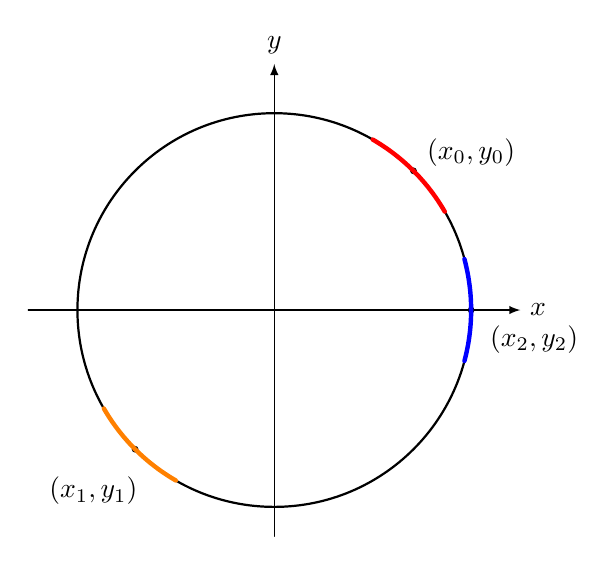
\begin{tikzpicture}[scale=2.5,cap=round,>=latex]
        % draw the coordinates
        \draw[->] (-1.25cm,0cm) -- (1.25cm,0cm) node[right,fill=white] {$x$};
        \draw[->] (0cm,-1.15cm) -- (0cm,1.25cm) node[above,fill=white] {$y$};

        % draw the unit circle
        \draw[thick] (0cm,0cm) circle(1cm);

        \filldraw[black] (45:1cm) circle(0.4pt)
                        (45:-1cm) circle(0.4pt)
                        (0:1cm) circle(0.4pt);

        \draw (1.32cm,-0.15cm) node(b) {$(x_2, y_2)$}
                        (1.0cm,0.8cm) node(a) {$(x_0, y_0)$}
                        (45:-1.3cm) node(c) {$(x_1, y_1)$};
                        
        \draw [red,ultra thick,domain=30:60] plot ({cos(\x)}, {sin(\x)});
        \draw [blue,ultra thick,domain=-15:15] plot ({cos(\x)}, {sin(\x)});
        \draw [orange,ultra thick,domain=210:240] plot ({cos(\x)}, {sin(\x)});
    \end{tikzpicture}
\end{center}
Если мы изобразим решения этого уравнения, то получится единичная окружность.
Зафиксируем на ней точку $(x_0, y_0)$. 
Если мы будем сдвигаться от нее немного влево и вправо, то у нас получится график функции.

Мы даже можем легко понять, как устроена эта функция: $g(x) = \sqrt{1 - x^2}$.
Так вот такая функция называется неявно заданной уравнением $x^2 + y^2 = 1$.

Если же мы зафиксируем точку $(x_1, y_1)$, то неявная функция примет вид $g(x) = -\sqrt{1 - x^2}$. 
А для точки $(x_2, y_2)$ это уже будет $h(y) = \sqrt{1 - y^2}$. 
Заметим, что для двух предыдущих точек мы также могли записать функцию для $y$.

Теорема о неявной функции как раз и говорит о том, в каком случае мы можем написать неявную функцию для конкретной переменной в конкретной точке.
